\documentclass[11pt,fleqn,a4paper,]{LegrandOrangeBook}
\addbibresource{sample.bib} % Bibliography file
\definecolor{ocre}{RGB}{243, 102, 25} 
\chapterimage{orange1.jpg} 
\chapterspaceabove{6.5cm}
\chapterspacebelow{6.75cm} 
%\begin{theorem}[Name of the theorem]
%\begin{exercise}
%\begin{example}[Example name]
%\begin{definition}[Definition name]
%\begin{corollary}[Corollary name]
%\begin{remark}
%\begin{proposition}[Proposition name]
%\begin{problem}
%\begin{vocabulary}[Word]
%----------------------------------------------------------------------------------------
\begin{document}
\section{Ley de Coulomb}\index{Ley de Coulomb}
La ley de Coulomb establece de la fuerza \textit{F} entre dos cargas \textit{$Q_1$} y \textit{$Q_2$} son:
\begin{itemize}
\item A lo largo de la linea que los une.
\item Directamemte proporcional al producto \textit{$Q_1Q_2$} de las cargas.
\item Inversamente proporcional a la distancia \textit{R} que los separa
\end{itemize}
\begin{theorem}[Ley de Coulomb]
\begin{equation}
\label{eq:eqCoulomb}
F=\frac{kQ_1Q_2}{R^2}
\end{equation}
Donde:\\
\begin{itemize}
\item \textit{Q}: Cargas en Coulombs(C).
\item R: Distancia en metros(m).
\item F: Fuerza Newtons(N).
\end{itemize}
Constantes:
\begin{align*}
&\epsilon_0=8.854 \times 10^{-12}\simeq \frac{10^{-9}}{36\pi}F/m
&k=\frac{1}{4\pi\epsilon_0}\simeq 9\times 10^9 m/F
\end{align*}
\end{theorem}
Si las cargas $\textit{Q}_1$ y $\textit{Q}_2$ están localizadas en puntos cuyas posiciones están de forma vectorial $\textit{r}_1$ y $\textit{r}_2$(figura ), así la fuerza de $\textbf{F}_{12}$\footnote{Se lee: La fuerza de la carga 1 a la carga 2} sobre la carga 2 debido a la carga 1 esta dado por:
\begin{multicols}{2}
\begin{equation}
\boxed{F_{12}=\frac{Q_1Q_2}{4\pi\epsilon_0R^2}\textbf{a}_{R_{12}}}
\end{equation}
Sean n cargas y se desea hallar la fuerza resultante en una carga Q, se usa el \textit{principio de superposición}. Este principio establece: Si existen N cargas $Q_1, Q_2,...,Q_N$ y seas sus vectores posición $r_1, r_2,.., r_N$ la fuerza resultante en la carga Q es la sumatoria de las fuerzas de cada una de las cargas:
\begin{displaymath}
F_Q=F_1+F_2+F_3+\ldots +F_N
\end{displaymath}
o:
\begin{equation}
\boxed{F=\frac{Q}{4\pi\epsilon_0}\sum^N_{k=1}\frac{Q_k(r-r_k)}{|r-r_k|^3}}
\end{equation}
\columnbreak
  \begin{center}
    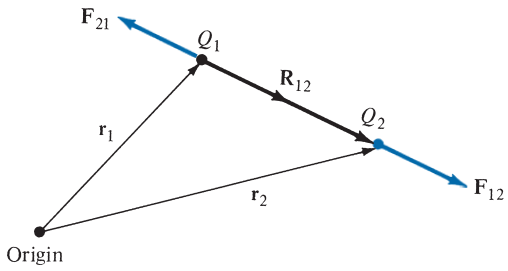
\includegraphics[scale=0.4]{CamposMag/CM10.png}
  \end{center}
\end{multicols}
\section{Intensidad de campo eléctrico}\index{Intensidad de campo eléctrico}
La intensidad de campo eléctrico E es la fuerza que una unidad de carga positiva experimenta cuando se coloca en un campo eléctrico.
\begin{theorem}[Intensidad de campo eléctrico]
\begin{equation}
\label{eq:Intensidadcampoelectrico}
E=\frac{F}{Q}
\end{equation}
Donde:
\begin{itemize}
\item E: Intensidad de campo eléctrico(N/C) o Volts por metro(V/m).
\item F: Fuerza(N)
\item Q: Carga(Coulombs).
\end{itemize}
\end{theorem}
Para Q>0, el E esta en la misma dirección de la fuerza F. La intensidad de campo eléctrico en el punto \textbf{r} debido a una carga localizada en \textbf{r'} es obtenido:
\begin{equation}
E=\frac{Q(r-r')}{4\pi\epsilon_0|r-r'|^3}=\frac{Q}{4\pi\epsilon_0r^2}a_r
\end{equation}
Y bajo el mismo principio de superposición, la intensidad de campo eléctrico en el punto \textbf{r}:
\begin{equation}
\boxed{E=\frac{1}{4\pi\epsilon_0}\sum^N_{k=1}\frac{Q_k(r-r_k)}{|r-r_k|^3}}
\end{equation}
\section{Campo eléctrico creado por una distribución continua de carga en un punto}\index{Campo eléctrico creado por una distribución continua de carga en un punto}
Las cargas puntuales ocupan un muy pequeño espacio físico. Es posible tener distribuciones continuas: Es costumbre denotar la densidad de carga lineal $\rho_L$(C/m), la densidad de carga superficial $\rho_S$(C/$m^2$) y la carga volumétrica $\rho_V$(C/$m^3$).\footnote{No confundir este $\rho$ con subíndice con $\rho$ sin subíndice usado en coordenadas cilíndricas.}
\begin{subequations}
\begin{align}
\label{eq:diferenciales de carga}
dQ=\rho_Ldl=\lambda dl &\rightarrow Q=\int_L\rho_Ldl\\
dQ=\rho_Sds=\sigma ds &\rightarrow Q=\int_S\rho_Sds\\
dQ=\rho_vdv=\rho dv &\rightarrow Q=\int_v\rho_vdv
\end{align}
\end{subequations}
El campo eléctrico debido a cada distribución de carga puede ser tomado como una sumatoria de los campos contribuidos por numerosas cargas:
\begin{subequations}
\begin{align}
\vec{E}&=\int_Lk\lambda\frac{dl}{r^2}\vec{u}_r\\
\vec{E}&=\int_Sk\sigma\frac{ds}{r^2}\vec{u}_r\\
\vec{E}&=\int_Vk\rho\frac{dv}{r^2}\vec{u}_r
\end{align}
\end{subequations}
\section{Densidad de campo eléctrico}\index{Densidad de campo eléctrico}
Se dice que la \textbf{densidad de flujo eléctrico} es el número de líneas de fuerza por metro cuadrado de superficie, para una esfera de radio \textit{r}, esta dada por:
\begin{equation}
\vec{D}=\frac{q}{4\pi r^2}\vec{r}
\end{equation}
Así para el espacio libre:
\begin{equation}
\vec{D}=\vec{E}\epsilon_0
\end{equation}
Donde:\\
\begin{itemize}
\item E: Campo eléctrico(N/C ó V/m).
\item D: Densidad de flujo eléctrico(C/$m^2$).
\end{itemize}
Se define \textbf{flujo eléctrico} en términos de la densidad de flujo eléctrico, es decir:
\begin{equation}
\Phi_{E}=\int_S\textbf{D}\cdot d\textbf{S}
\end{equation}
Otra forma de ver el flujo eléctrico(figura \ref{fig:flujo electrico en la superficie}), solo si las lineas de campo eléctrico uniforme atraviesan una superficie de área \textit{S} es:
\begin{equation}
\label{eq:flujo coseno}
\Phi=ES\cos\theta
\end{equation}
Donde:\\
\begin{itemize}
\item E: Campo eléctrico.
\item S: Área de la superficie.
\item $\theta$: Angulo que forman los vectores de campo eléctrico y la normal de la superficie
\end{itemize}
\begin{figure}[h!]
\centering
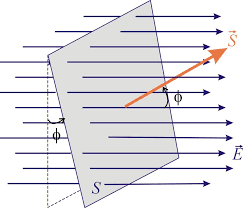
\includegraphics[scale=0.5]{CamposMag/CM11.png}
\caption{Flujo eléctrico}
\label{fig:flujo electrico en la superficie}
\end{figure}
\section{Ley de Gauss-Ecuaciones de Maxwell}\index{Ley de Gauss-Ecuaciones de Maxwell}
La ley de Gauss establece que el flujo a través de una superficie que no encierra carga es nulo, en este caso el número neto de líneas de campo que atraviesa la superficie es cero (entran el mismo número de líneas que salen). Por otro lado, el flujo eléctrico total $\Phi_{E}$ a traves de la \textbf{superficie cerrada} es igual a la carga total encerrada por la superficie.\\

Por lo tanto:
\begin{displaymath}
\Phi_{E}=Q_{enc}
\end{displaymath}
que es:
\begin{displaymath}
\Phi_{E}=\oint_s d\Phi_{E} = \oint_s D\cdot dS
\end{displaymath}
La carga total encerrada:
\begin{equation}
\label{eq:cargaintegral}
Q=\oint D\cdot dS=\int_v\rho_vdv
\end{equation}
Aplicando el teorema de la divergencia al término medio.
\begin{equation}
\label{eq:cargaintegral1}
\oint D\cdot dS = \int_v\nabla\cdot D dv
\end{equation}
¿Qué pasa si $\vec{E}$ no es uniforme o si \textit{S} es una superficie general?\\
Si queremos calcular el flujo eléctrico se calcula dividendo el área en diferenciales de área, y usando la ecuación \ref{eq:flujo coseno} se suma todas las pequeñas partes:
\begin{displaymath}
\Phi_E=\sum^{\infty}_{i=1}\vec{E_i}\Delta\vec{A_i}
\end{displaymath}
Que puede ser expresada como una integral de superficie(ecuación \ref{eq:leydemaxwell1int})
\begin{theorem}[Ley de Gauss]
El flujo eléctrico que pasa a través de cada superficie gaussiana\footnote{Se llama superficie gaussiana a la superficie \textbf{imaginaria} que encierra las cargas a analizar, no siempre tiene que coincidir necesariamente con la distribución de carga.} es igual a la carga neta encerrada(suma de las cargas encerradas) entre la \textit{permisividad en el vacío} Comparando los volúmenes de las dos integrales(ecuación \ref{eq:cargaintegral} y \ref{eq:cargaintegral1}):\\
\textbf{Forma diferencial:}
\begin{equation}
\label{eq:leydemaxwell1der}
\boxed{\nabla\cdot\vec{D}=\rho_v}
\end{equation}
\begin{equation}
\label{eq:leydemaxwell1}
\boxed{\vec{\nabla}\cdot\vec{E}=\frac{\rho}{\epsilon_0}}
\end{equation}
\textbf{Forma integral:}
\begin{equation}
\label{eq:leydemaxwell1int}
\boxed{\Phi_{E}=\oint_s\vec{E}\cdot d\vec{A}=\frac{Q_{enc}}{\epsilon_0}}
\end{equation}
Las ecuaciones \ref{eq:leydemaxwell1}, \ref{eq:leydemaxwell1der} y \ref{eq:leydemaxwell1int} son la primera de la 4 ecuaciones de Maxwell establece:\\
\textit{Que el volumen de densidad de carga es la misma que la divergencia de la densidad de flujo eléctrico. Es equivalente a la ley de Coulomb de fuerza entre dos cargas}.
\end{theorem}
\begin{itemize}
\item La ley de Gauss es útil cuando se demuestra por simetría el valor de campo eléctrico es constante sobre nuestra superficie gaussiana.
\item Ademas el vector normal $d\vec{A}$ siempre apunta hacia afuera del volumen encerrado por la superficie cerrada, es necesario decir que no siempre el campo eléctrico no apuntara a una dirección, depende de la carga, si es positiva será hacia afuera del volumen y si es negativa será hacia adentro de la superficie.
\item Si $\vec{E}$ es \textbf{tangente} a la superficie gaussiana en cada punto, entonces la integral sobre la superficie es cero.
\end{itemize}
La ley de Gauss tambien puede ser usada para distribuciones de carga no uniforme es necesario una densidad de carga del cuerpo en estudio varíe según una coordenada espacial y para calcular el campo eléctrico primero se debe calcular la carga encerrada por la superficie gaussiana(ecuaciones \ref{eq:diferenciales de carga}).
%----------------------------------------------------------------------------------------
\end{document}